\documentclass[conference]{IEEEtran}
\usepackage{cite}
\usepackage{amsmath,amssymb,amsfonts}
\usepackage{algorithmic}
\usepackage{algorithm}
\usepackage{graphicx}
\usepackage{textcomp}
\usepackage{xcolor}
\usepackage{listings}
\usepackage{booktabs}
\usepackage{hyperref}
\usepackage{tabularx}
\usepackage{multirow}
\usepackage{tikz}
\usetikzlibrary{arrows.meta,positioning}

\lstset{
  basicstyle=\ttfamily\footnotesize,
  breaklines=true,
  frame=single,
  numbers=none,
  xleftmargin=2mm,
  xrightmargin=2mm,
  aboveskip=4pt,
  belowskip=4pt,
  columns=fullflexible,
  keepspaces=true
}

\begin{document}

\title{Error-Guided Repair for Compiler Fuzzing:\\A Completion-Style Extension to Fuzz4All}

\author{\IEEEauthorblockN{Aniket Salunke}
\IEEEauthorblockA{CS7602 / CS8602\\
Mohamed bin Zayed University of Artificial Intelligence\\
aniket.salunke@mbzuai.ac.ae}}

\maketitle

\begin{IEEEkeywords}
Fuzz4All, compiler fuzzing, large language models, error-guided repair, completion-style prompting, StarCoderBase.
\end{IEEEkeywords}

% ===================================================================
\begin{abstract}
Large Language Models have shown strong potential as universal fuzzers for compiler testing. However, Fuzz4All~\cite{xia2024fuzz4all} discards all programs that fail to compile---typically 40--60\% of generated inputs---wasting significant inference compute. We propose an \emph{error-guided repair} stage that intercepts compilation failures, feeds the compiler's diagnostic output back to the generation LLM, and attempts to produce a corrected program. Rather than requiring paid instruction-following models, our approach reformulates repair prompts in a \emph{completion-style} format compatible with open-weight code-completion LLMs such as StarCoderBase~\cite{starcoder}. We treat repair hyperparameter selection (template, error gate, attempt budget) as an adaptive search problem over candidate configurations with a fixed evaluator and measurable improvement metrics. Evaluation on 200 C++ programs targeting \texttt{g++} shows that the repair stage recovers 45.9\% of compilation failures, improving the overall valid rate from 60.5\% (baseline) to 73.5\% (+13 percentage points) using StarCoderBase-7B, with no external API dependencies.
\end{abstract}

% ===================================================================
\section{Paper Context and Threat Model}
% ===================================================================

\subsection{Paper Context}

Xia et al.~\cite{xia2024fuzz4all} present Fuzz4All, a universal fuzzer that leverages Large Language Models to generate test inputs for compilers, runtime engines, and constraint solvers. The system operates in two stages: (1)~an \emph{autoprompting} stage that uses GPT-4 to distill user-provided documentation into an effective generation prompt, and (2)~an \emph{LLM-powered fuzzing loop} with three generation strategies: \texttt{generate}, \texttt{mutate}, and \texttt{semantic-equiv}. The generation LLM is StarCoder (15B parameters), a decoder-only code-completion model trained on over one trillion tokens of permissively-licensed code.

For C++ compiler fuzzing, Fuzz4All generates programs and validates them using a compile-only oracle (\texttt{g++ -c}). Programs that fail to compile are \emph{discarded}. Across nine systems under test (SUTs), the paper reports 36.8\% average coverage improvement and 98 bugs (64 confirmed). However, for C++ specifically, only 40.7\% of generated programs are valid---meaning nearly 60\% of all LLM inference is wasted on unusable outputs.

\subsection{Threat Model}

We adopt the standard compiler fuzzing threat model:
\begin{itemize}
    \item \textbf{System under test (SUT):} GNU C++ compiler (\texttt{g++ 11}), invoked in compile-only mode: \texttt{g++ -x c++ -std=c++23 -O0 -c}.
    \item \textbf{Oracle:} Deterministic---a program either compiles (OK) or produces a classified failure (COMPILE\_ERROR, ICE, CRASH, TIMEOUT).
    \item \textbf{Safety invariant:} The compiler should never crash or produce an internal compiler error (ICE) on any input, including syntactically invalid programs.
    \item \textbf{Attacker model:} The fuzzer generates adversarial C++ source files at inference time using an open-weight LLM. No model fine-tuning or paid API access is permitted.
\end{itemize}

\subsection{Focus and Justification}

We focus on the \emph{generation validity bottleneck}: the fraction of generated programs that fail to compile and are currently discarded. This is the right slice because (a)~it directly affects fuzzing throughput---more valid programs means more opportunities to trigger compiler bugs, (b)~the wasted inference is the dominant cost in LLM-based fuzzing, and (c)~compiler error messages provide structured, machine-readable feedback that can guide targeted repair.

\begin{figure}[t]
\centering
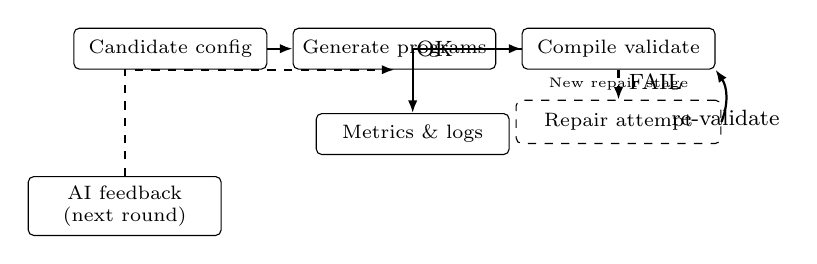
\begin{tikzpicture}[
  font=\scriptsize,
  node distance=0.28cm and 0.32cm,
  box/.style={rectangle, draw, rounded corners=2pt, minimum width=2.45cm, minimum height=0.52cm, align=center},
  repbox/.style={rectangle, draw, dashed, rounded corners=2pt, minimum width=2.6cm, minimum height=0.55cm, align=center},
  arr/.style={-{Latex[length=1.6mm]}, thick}
]
\node[box] (cfg) {Candidate config};
\node[box, right=of cfg] (gen) {Generate programs};
\node[box, right=of gen] (val) {Compile validate};
\node[box, below left=0.55cm and 0.15cm of val] (met) {Metrics \& logs};
\node[repbox, below=0.38cm of val, label=above:{\tiny New repair stage}] (rep) {Repair attempt};
\node[box, below left=1.35cm and 0.9cm of gen] (ai) {AI feedback\\(next round)};

\draw[arr] (cfg) -- (gen);
\draw[arr] (gen) -- (val);
\draw[arr] (val) -| node[near start, left, xshift=-0.05cm] {\footnotesize OK} (met.north);

\draw[arr, dashed] (val.south) -- node[right, pos=0.42] {\footnotesize FAIL} (rep.north);
\draw[arr] (rep.east) to[bend right=28] node[below, yshift=-0.06cm] {\footnotesize re-validate} (val.south east);

\draw[arr, dashed] (ai.north) |- (gen.south);
\end{tikzpicture}
\caption{System overview. The extension adds error-guided repair (and optional search over candidates) on top of baseline Fuzz4All: failed compilations are repaired and re-validated; structured logs feed AI-assisted candidate refinement.}
\label{fig:overview}
\end{figure}

% ===================================================================
\section{Project Problem}
% ===================================================================

\subsection{Sub-Problem Definition}

\textbf{Objective:} Design an error-guided repair stage that maximizes the fraction of compilable programs produced by the fuzzing loop, without requiring external APIs or model fine-tuning.

Given a fixed generation budget of $N$ programs, let $V$ denote the number of valid (compilable) programs and $F = N - V$ denote the failures. The baseline discards all $F$ programs. We introduce a repair function $R$ that attempts to convert failures into valid programs:
\[
V^{*} = V + \sum_{i=1}^{F} \mathbf{1}\big[R(p_i, \texttt{stderr}_i) \text{ compiles OK}\big]
\]

\textbf{Success criteria:} Valid rate $V^*/N$ exceeds baseline $V/N$ by a statistically meaningful margin ($\Delta \geq 0.05$) on a budget of $N = 200$ programs. Repair success rate $S/A \geq 0.20$ (at least 20\% of attempted repairs succeed).

\textbf{Constraints:} (1)~No paid APIs; reuse the existing local LLM. (2)~Single SUT: \texttt{g++}, compile-only. (3)~Must not degrade baseline when repair is disabled. (4)~Must run on HPC (no Docker).

\subsection{Why It Is Non-Trivial}

\textbf{1. Prompt--Model Mismatch.} Code-completion LLMs such as StarCoder are \emph{not} instruction-following models. Standard repair prompts (``Fix the following program...'') produce unrelated code continuations rather than targeted fixes. We experimentally confirm this: instruction-style prompts yield 0\% repair success with StarCoderBase-7B (Sec.~\ref{sec:prelim}). Reformulating repair as a code-completion problem is non-obvious and requires careful prompt engineering.

\textbf{2. Error Diversity.} Compiler errors span a wide range: missing includes, type mismatches, template instantiation failures, preprocessor errors, duplicate definitions. Each error category may require a different repair strategy. A single prompt template cannot address all categories effectively.

\textbf{3. Cost--Benefit Tradeoff.} Each repair attempt consumes an additional LLM inference call ($\sim$6s per attempt on our hardware). If repair success rate is low, the added compute may outweigh the benefit. The optimal configuration (template, error gate, max attempts) depends on model capability, prompt design, and error distribution---creating a non-trivial search space.

\subsection{Novelty Over Baseline}

Fuzz4All has no feedback loop for failed programs. Our extension introduces:
\begin{itemize}
    \item \textbf{Structured validation}: Five-category classification (OK, COMPILE\_ERROR, ICE, CRASH, TIMEOUT) with normalized error signatures for clustering.
    \item \textbf{Completion-style repair prompts}: A prompt format presenting broken code as comments and seeding the completion with the first \texttt{\#include} directive, compatible with decoder-only LLMs.
    \item \textbf{Signature-based caching}: Normalized failure signatures as cache keys to avoid redundant LLM calls for repeated error patterns.
    \item \textbf{Configurable repair pipeline}: Six prompt templates (T1--T6) and multiple error gates, exposing a candidate space for systematic search.
\end{itemize}

% ===================================================================
\section{Candidates, Evaluator, and Metrics}
% ===================================================================

\subsection{Candidate Representation}

Each candidate configuration is a JSON object specifying generation and repair hyperparameters:

\begin{lstlisting}
{"name": "c1",
 "gen": {"llm": {"batch_size": 4}},
 "repair": {
   "enabled": true,
   "max_attempts": 2,
   "template_id": "T1",
   "error_gate": "compile_error",
   "cache": true,
   "max_tokens": 256,
   "temperature": 0.7
 }}
\end{lstlisting}

\noindent The candidate space includes:
\begin{itemize}
    \item \textbf{Template ID}: T1 (minimal patch), T2 (include/namespace focus), T3 (type/template fix), T4 (local simplification), T5 (structure-preserving), T6 (timeout defense).
    \item \textbf{Error gate}: \texttt{compile\_error}, \texttt{ice}, \texttt{crash}, \texttt{all\_non\_timeout}.
    \item \textbf{Max attempts}: 1--3 repair attempts per failure.
    \item \textbf{Temperature}: 0.3--1.0 for repair generation.
\end{itemize}

Three initial candidates define the first search round:
\begin{itemize}
    \item \textbf{c1}: repair ON, T1, batch\_size=10, 1 attempt
    \item \textbf{c2}: repair ON, T2, batch\_size=5, 2 attempts
    \item \textbf{c3}: repair OFF (baseline control)
\end{itemize}

\subsection{Evaluator}

The evaluator is a deterministic function implemented as \texttt{evaluate\_candidate.py}:

\begin{lstlisting}
evaluate(candidate, N, R) -> {
  summary.csv,        # one row per repeat
  summary_mean_std.json  # mean +/- std
}
\end{lstlisting}

\noindent\textbf{Procedure:}
\begin{enumerate}
    \item Materialize candidate JSON into a YAML configuration file.
    \item Run the fuzzing pipeline with a fixed program budget~$N$.
    \item For each generated program, compile with \texttt{g++ -c -std=c++23}.
    \item On compilation failure, if repair is enabled and \texttt{should\_repair()} returns true, attempt up to \texttt{max\_attempts} independent repairs.
    \item Write per-program JSONL records and aggregate run-level metrics.
    \item Repeat $R$ times; compute mean $\pm$ std across repeats.
\end{enumerate}

\noindent\textbf{Inputs:} candidate config (YAML), program budget~$N$, number of repeats~$R$, target binary path.\\
\textbf{Outputs:} per-run \texttt{records.jsonl}, \texttt{metrics.json}, \texttt{repair\_cache.json}; across-run \texttt{summary.csv} and \texttt{summary\_mean\_std.json}.\\
\textbf{Repeatability:} Same model weights + config produce comparable distributions; we report mean $\pm$ std over $R$ repeats.

\subsection{Structured Validation Pipeline}

Each program validation produces a structured \texttt{ValidationResult}:

\begin{lstlisting}
ValidationResult {
  status: OK | COMPILE_ERROR | ICE
        | CRASH | TIMEOUT
  exit_code: int
  elapsed_sec: float
  stderr: str  (truncated: 20 lines, 4KB)
  signature: str (normalized fingerprint)
}
\end{lstlisting}

\noindent Signature normalization strips absolute paths, line/column numbers, and temp filenames, retaining only the error category and key diagnostic text. This enables clustering of repeated failure patterns.

We present three representative outputs from our 200-program evaluation:

\textbf{1) Compilation success (no repair needed):}
\begin{lstlisting}
{"program_id": 0, "is_repair": false,
 "compile_status": "OK", "exit_code": 0,
 "elapsed_sec": 0.276}
\end{lstlisting}

\textbf{2) Failure $\to$ repair succeeds (attempt 1):}
\begin{lstlisting}
{"program_id": 25, "is_repair": false,
 "compile_status": "COMPILE_ERROR",
 "signature": "error: #endif without #if"}
{"program_id": 25, "is_repair": true,
 "repair_attempt_index": 1,
 "compile_status": "OK", "exit_code": 0}
\end{lstlisting}

The original program contained an orphan \texttt{\#endif} directive. The repair LLM produced a corrected version wrapping the problematic code in a proper \texttt{\#if 0 / \#endif} guard.

\textbf{3) Failure $\to$ repair fails (both attempts):}
\begin{lstlisting}
{"program_id": 4, "is_repair": false,
 "compile_status": "COMPILE_ERROR",
 "signature": "error: #endif without #if"}
{"program_id": 4, "is_repair": true,
 "repair_attempt_index": 1,
 "compile_status": "COMPILE_ERROR"}
{"program_id": 4, "is_repair": true,
 "repair_attempt_index": 2,
 "compile_status": "COMPILE_ERROR"}
\end{lstlisting}

\subsection{Metrics}

Let $N$ be total programs generated, $V$ the number compiled OK (including repaired), $U$ the unique valid programs (by SHA-256 hash), $A$ the repair attempts, and $S$ the successful repairs.

\textbf{Primary metrics:}
\begin{align}
V_r &= V / N && \text{(valid rate)} \\
U_r &= U / N && \text{(unique valid rate)} \\
R_s &= S / A && \text{(repair success rate)} \\
\Delta &= V_r^{\text{repair}} - V_r^{\text{baseline}} && \text{(improvement)}
\end{align}

\textbf{Cost metrics:}
\begin{itemize}
    \item \textbf{Avg time/program}: Wall-clock time including validation + repair. Baseline: 0.247s; Repair: 6.65s (27$\times$ overhead).
    \item \textbf{LLM overhead}: Total LLM calls / max($V$, 1). Baseline: 0.41; Repair: 1.26.
    \item \textbf{False positives}: A repaired program compiles but is semantically trivial (e.g., empty body). Mitigated by prompt templates that preserve program structure.
    \item \textbf{False negatives}: Repairable failures the system cannot fix. Measured as $1 - R_s$.
\end{itemize}

\textbf{Interpretation:} $\Delta > 0$ means repair improves yield; $\Delta = 0$ means no effect; $\Delta < 0$ means overhead exceeds benefit (fallback to baseline).

\noindent\textbf{Scope of metrics:} We optimize \emph{valid-input yield} at the compile stage (oracle: \texttt{g++ -c}). We do not yet measure downstream compiler bug discovery or differential testing; higher $V_r$ is a prerequisite for those stages.

\subsection{Preliminary Results}
\label{sec:prelim}

\begin{table}[t]
\centering
\caption{Pilot evaluation: baseline vs.\ repair (T1), 200 programs, StarCoderBase-7B, \texttt{g++ -c -std=c++23}}
\label{tab:main_results}
\begin{tabular}{lcc}
\toprule
\textbf{Metric} & \textbf{Baseline} & \textbf{Repair (T1)} \\
\midrule
Total compiled OK & 121 & \textbf{147} \\
Valid rate ($V_r$) & 0.605 & \textbf{0.735} \\
Unique valid rate ($U_r$) & 0.485 & \textbf{0.690} \\
Duplicate rate & 0.120 & 0.045 \\
\midrule
Repair attempted ($A$) & --- & 98 \\
Repair succeeded ($S$) & --- & \textbf{45} \\
Repair success rate ($R_s$) & --- & \textbf{0.459} \\
\midrule
Avg time/program (s) & 0.247 & 6.650 \\
LLM overhead & 0.413 & 1.259 \\
\bottomrule
\end{tabular}
\end{table}

The repair stage recovers 45 of 98 failures (45.9\% success rate), improving the valid rate by $\Delta = +0.13$ (60.5\% $\to$ 73.5\%). The unique valid rate improves by $+0.205$ (48.5\% $\to$ 69.0\%), indicating repaired programs add genuine diversity. We exceed both success criteria ($\Delta = 0.13 > 0.05$; $R_s = 0.459 > 0.20$).

\textbf{Key finding:} Prompt format is critical. An earlier experiment using instruction-style prompts (``Fix the following C++ program'') with the same 7B model achieved \textbf{0\% repair success}---the completion model generated unrelated continuations. Reformulating prompts in completion style (presenting broken code as C++ comments and seeding the output with the first \texttt{\#include}) increased success to 45.9\%.

% ===================================================================
\section{AI / Search Strategy}
% ===================================================================

\subsection{Search Formulation}

We formulate repair hyperparameter selection as an adaptive search over a candidate space $\mathcal{C}$. At each round $n$, the system evaluates $k$ candidates using the fixed evaluator and generates structured feedback for proposing the next round.

\subsection{Architecture}

The search loop consists of four components:

\begin{enumerate}
    \item \textbf{Candidate Generator}: Produces JSON candidates specifying generation and repair parameters. Initial candidates are hand-crafted; subsequent rounds are proposed by an AI assistant consuming structured feedback.
    \item \textbf{Evaluator} (\texttt{evaluate\_candidate.py}): Runs the fuzzing pipeline with fixed budget $N$ and computes metrics.
    \item \textbf{Search Logger} (\texttt{search\_log.jsonl}): Appends per-candidate \{name, metrics\_mean, metrics\_std\} for cumulative tracking across rounds.
    \item \textbf{Feedback Synthesizer} (\texttt{next\_prompt.md}): Generates a structured report containing:
    \begin{itemize}
        \item Ranked table of all candidates by $V_r$
        \item Common failure signature clusters (top-15 by frequency)
        \item Explicit instruction: ``Propose the next round of candidates in the same JSON format''
    \end{itemize}
\end{enumerate}

The feedback file is designed to be copy-pasted into an AI assistant (ChatGPT, Cursor) to propose the next round. This enables a human-in-the-loop search loop without any paid API calls from the codebase itself.

\begin{figure}[h]
\centering
\fbox{\begin{minipage}{0.92\columnwidth}
\scriptsize
\texttt{\# excerpt from next\_prompt.md}\\[0.3em]
Top candidates: c2 ($V_r{=}0.70$), c1 ($V_r{=}0.50$). Common signatures: \emph{\#endif without \#if}, template mismatch, missing include.\\[0.2em]
\textit{Instruction:} Propose 3 new JSON candidates varying template\_id, max\_attempts, or error\_gate; keep one repair-off control.
\end{minipage}}
\caption{Example structure of AI-facing feedback (human-in-the-loop; no API in code).}
\label{fig:feedback}
\end{figure}

\subsection{Pruning and Selection Rules}

\begin{itemize}
    \item \textbf{Ranking}: Candidates are ranked by valid rate $V_r$. Top-$k$ ($k=2$) are retained as seeds for the next round.
    \item \textbf{Baseline guard}: Any candidate with $V_r < V_r^{\text{baseline}}$ is flagged for removal.
    \item \textbf{Control arm}: At least one candidate per round has repair disabled, to detect regression.
    \item \textbf{Diversity}: Each new candidate must vary at least one axis (template, gate, attempts, temperature) from existing candidates.
    \item \textbf{Stopping}: Terminate after 3 rounds or when $\Delta_n < 0.02$ for two consecutive rounds.
\end{itemize}

\subsection{Algorithm}

\begin{algorithm}[h]
\caption{Error-Guided Repair Search Loop}
\begin{algorithmic}[1]
\STATE \textbf{Input:} base config $C_0$, budget $N$, max rounds $R$
\STATE Load initial candidates from \texttt{round\_01.json}
\FOR{$n = 1$ to $R$}
    \FOR{each candidate $c_i$ in round $n$}
        \STATE Materialize YAML: merge $C_0$ with $c_i$ overrides
        \STATE $m_i \leftarrow$ \texttt{evaluate}($c_i$, $N$, repeats=1)
        \STATE Append $\{c_i.\text{name}, m_i\}$ to \texttt{search\_log.jsonl}
    \ENDFOR
    \STATE Rank candidates by $V_r$; mark below-baseline
    \STATE Generate \texttt{next\_prompt.md} with ranked table + failure clusters
    \IF{$|\Delta_n| < 0.02$ for 2 consecutive rounds}
        \STATE \textbf{break} \COMMENT{plateau detected}
    \ENDIF
    \STATE Copy \texttt{next\_prompt.md} to AI $\to$ get \texttt{round\_0\{n+1\}.json}
\ENDFOR
\STATE \textbf{Return} best candidate by $V_r$
\end{algorithmic}
\end{algorithm}

\subsection{Round 1 Results}

Table~\ref{tab:search_r1} validates the \emph{search harness infrastructure} (materialize YAML, evaluate, log, emit \texttt{next\_prompt.md}) using a smaller 1B model for speed. Table~\ref{tab:main_results} reports the main repair effect with StarCoderBase-7B and $N{=}200$.

\begin{table}[t]
\centering
\caption{Search harness: three candidates, 10 programs each (StarCoderBase-1B)}
\label{tab:search_r1}
\begin{tabular}{lcccc}
\toprule
\textbf{Name} & $V_r$ & $R_s$ & \textbf{LLM OH} & \textbf{Time/prog} \\
\midrule
c2 (T2, 2 att.) & \textbf{0.70} & 0.00 & 0.29 & 0.24s \\
c1 (T1, 1 att.) & 0.50 & 0.00 & 0.60 & 0.30s \\
c3 (no repair) & 0.30 & --- & 0.33 & 0.24s \\
\bottomrule
\end{tabular}
\end{table}

The 1B model was too small to produce useful repairs ($R_s = 0$), but the pipeline correctly evaluated all candidates, logged structured metrics, and generated \texttt{next\_prompt.md} with failure signature clusters. Upgrading to the 7B model (Table~\ref{tab:main_results}) shows non-zero $R_s$ when prompts match the completion model (Sec.~\ref{sec:prelim}).

% ===================================================================
\section{Scope and Assumptions}
% ===================================================================

\textbf{Explicit exclusions and justifications:}
\begin{itemize}
    \item \textbf{Single SUT}: We target only \texttt{g++}, compile-only mode. Generalization to other compilers (Clang, MSVC) or languages (Java, Go) is structurally supported by the modular design but not evaluated. \emph{Justification}: A single SUT is sufficient to validate the repair concept; the candidate--evaluator--search architecture generalizes without structural changes.
    \item \textbf{Reduced model}: We use StarCoderBase-7B (7B parameters) rather than the 15B model from the original paper. Our GPU (32\,GB VRAM) could not sustain the 15B model reliably during extended runs. \emph{Justification}: The 7B model is the largest that fits stably; the repair mechanism is model-agnostic.
    \item \textbf{Small budget}: $N = 200$ programs per run, versus 26{,}000+ in the original paper. \emph{Justification}: Sufficient to demonstrate the repair mechanism and measure $\Delta$ with meaningful signal, within HPC time constraints ($\sim$48 minutes per run).
    \item \textbf{Compile-only oracle}: We do not perform differential testing or runtime-behavior analysis. \emph{Justification}: The validity bottleneck (60\% failure rate) exists at the compile stage; addressing it is prerequisite to any downstream oracle.
    \item \textbf{Human-in-the-loop search}: The search harness generates structured feedback for manual copy-paste to an AI assistant, rather than autonomous API calls. \emph{Justification}: Satisfies the ``no paid API'' constraint while still enabling systematic, iterative candidate refinement.
\end{itemize}

\textbf{Threat-model assumptions:}
\begin{itemize}
    \item The compiler oracle is deterministic and fast ($<$1s per invocation).
    \item The LLM produces diverse outputs across temperature-scaled generations.
    \item The repair function does not need to preserve \emph{semantic} behavior---only syntactic compilability.
\end{itemize}

% ===================================================================
\section{Feasibility and Risks}
% ===================================================================

\subsection{Resource Budget}

\begin{itemize}
    \item \textbf{Hardware}: NVIDIA RTX 5000 Ada Generation (32\,GB VRAM), 250\,GB RAM, 24 CPU cores (MBZUAI HPC workstation node).
    \item \textbf{Model}: StarCoderBase-7B, FP16 ($\sim$14\,GB VRAM). Batch size 4 fits within GPU memory.
    \item \textbf{Time per run}: Baseline 200 programs $\approx$ 25 min; Repair 200 programs $\approx$ 48 min. A full search round (3 candidates) completes in $<$3 hours.
    \item \textbf{Storage}: Each run produces $\sim$2\,MB of logs (\texttt{.fuzz} files + JSONL + JSON). 10 runs $\approx$ 20\,MB.
    \item \textbf{Dependencies}: Python 3.10, PyTorch, HuggingFace Transformers. No Docker, no paid APIs.
\end{itemize}

\subsection{Key Risks and Mitigations}

\begin{table}[t]
\centering
\caption{Key risks and mitigations}
\label{tab:risks}
\begin{tabular}{p{0.22\columnwidth}p{0.68\columnwidth}}
\toprule
\textbf{Risk} & \textbf{Mitigation} \\
\midrule
GPU OOM & Batch size configurable; tested stable at 4 for 7B. Fallback: reduce to batch\_size=1 or use 1B model. \\
\addlinespace
Repair loop divergence & Hard cap: \texttt{max\_attempts} $\leq$ 3. Each attempt is independent (fresh LLM call). \\
\addlinespace
Prompt--model mismatch & Validated: instruction prompts $\to$ 0\% success; completion prompts $\to$ 45.9\%. \\
\addlinespace
HPC time limits & Small budgets ($N = 200$); \texttt{tmux} for persistence; 5s per-program timeout. \\
\addlinespace
Evaluator instability & Fixed evaluator code; deterministic oracle; metrics schema frozen. \\
\bottomrule
\end{tabular}
\end{table}

\subsection{Fallback Plan}

If the repair stage degrades overall performance ($\Delta < 0$):
\begin{enumerate}
    \item Disable repair (\texttt{repair.enabled: false}) to revert to exact baseline.
    \item Restrict error gate to \texttt{compile\_error} only (exclude ICE/CRASH).
    \item Reduce \texttt{max\_attempts} to 1 to minimize compute overhead.
    \item Substitute StarCoderBase-1B for faster iteration during search.
\end{enumerate}

The system design guarantees that disabling repair produces identical behavior to the original Fuzz4All, as repair code is gated behind \texttt{if repair\_config.enabled}.

% ===================================================================

\begin{thebibliography}{2}

\bibitem{xia2024fuzz4all}
C.~S.~Xia, M.~Paltenghi, J.~L.~Tian, M.~Pradel, and L.~Zhang, ``Fuzz4All: Universal Fuzzing with Large Language Models,'' in \emph{Proc.\ ICSE}, 2024, pp.~1--13. Available: \url{https://github.com/fuzz4all/fuzz4all}

\bibitem{starcoder}
R.~Li \emph{et al.}, ``StarCoder: May the Source Be With You!,'' \emph{arXiv preprint arXiv:2305.06161}, 2023.

\end{thebibliography}

\end{document}
